\graphicspath{{mechanism/}}

\chapter{Teaching the Mechanism of the Greenhouse Effect}
\label{chap:mechanism}

As described above, American's lag much of the world regarding acceptance of
anthropogenic climate change. Informally, Michael Ranney, then other members of
our group started questioning whether people were able to mechanistically
explain how human activities cause an increase in global mean temperature.
Almost no one could provide a satisfactory explanation, including us! Prof.
Ranney, Lloyd Goldwasser, and Daniel Reinholz (along with input from myself and
Ronald Cohen) proceeded to develop a short \~400-word description of the
mechanism. This text is reproduced in full in Appendix~\ref{app:400words}.
Before reading the text yourself, I would encourage you to spend 10 minutes
describing \emph{your} understanding either aloud or on paper.
\footnote{If you personally doubt the veracity of anthropogenic climate change,
    then you may modify the exercise to describing the mechanism of the
    greenhouse effect, first described by Nobel laureate XXX Ahreneous (Sp?) in
    \citeyear{Ahreneous} (and accepted as fact since that time!).}

Given that our informal investigations implied that almost no-one knew the basic
concepts described in our 400 words, we initiated the line of research described
below. In these experiments, we sought to formally ask:

\begin{enumerate}
\item Is this lack of understanding for the mechanism of global climate change
    as pervasive as it seemed to be?
\item Does instruction regarding the mechanism of global climate change increase
    individuals' acceptance of the reality of anthropogenic climate change?
\end{enumerate}
Along the way, we additionally considered related aspects of learners'
cognition (the details of which are described below).

The history of educational research would imply that it’s quite difficult to
arrive at definitive answers to big policy qeustions. For example, phonics vs.
whole-word reading has been debated at least since the dawn of the Common Era,
as discussed in \textcite{history-reading-instruction}. Below, however, I report
on a series of experiments that argue strongly (if not definitively!) that
instruction regarding the pysical mechanism of the greenhouse effect appears to
have some positive effect on public acceptance of anthropogenic climate change.
As discussed above, such public acceptance seems central to any truly democratic
approach to the problem of climate change.

Others’ studies noted above detract from the utility of approaching climate
change as a science education problem. However, unlike those studies, the
interventions in this chapter have focused on a fundamental, well-researched
knowledge gap, and our assessment focused on acceptance/belief. Such contrasts
may explain the difference between observing instructional benefits (as we have)
or polarization (as others occasionally have; cf. Lundmark, 2007). We'll see
further evidence below, however, that such interventions are applicable across a
variety of settings, time-frames, and populations, and that global warming
understandings and attitudes are far from static. Most importantly, such
understandings seem to affect attitudes and beliefs in a meaningful way.

\section{Introducing our survey methods}
\label{sec:survey}

This chapter, as well as Chapters~\ref{chap:evilndi} and \ref{chap:prondi} all
utilize similar survey methods to assess climate-related beliefs and attitudes,
in addition to a number of related constructs relevant to Ranney's
(\citeyear{ranney_why_2012}) RTMD theory. For reference, the full list of survey
items used in this body of research is included in
Appendix~\ref{app:survey-items}. Below, we'll examine the way our interventions
are able to shift these beliefs and attitudes (primarily those related to
climate change), as well as noting how these beliefs and attitudes relate to one
another.  And, I hasten to note, the number of potential relationships between
the many variables we have measured would require an enormous amount of data to
test fully. As such, we will restrict ourselves primarily to the exploration of
\emph{a priori} relationships of interest.

\subsection{Clarifying \texorpdfstring{“beliefs”}{"beliefs"} and
    \texorpdfstring{“attitudes”}{"attitudes"}}

Survey methods in the social sciences may use the terms “belief” and “attitude”
in numerous ways. For example, an “attitude” may refer to a measured response,
whereas a “belief” may refer to a latent variable that explains a number of such
responses \cite{attitude-latent-var-ref}. Here, we take a more common-language
approach. Specifically, in the text that follows, a “belief” is a measure of
agreement with an objectively verifiable fact about the world (For example. For
example, the reality of anthropogenic climate change (item \textsf{gw1_2}) may
be difficult to ascertain, but in the end, it is something that could be settled
by observation. An “attitude,” on the other hand, is a measure of agreement with
an emotional stance towards some aspect of the world. For example, worry about
global warming (\textsf{gw2_3}).

\subsection{An overview of survey items}

Survey items were primarily sourced from \textcite{martinez_factors_2009}, and
were chosen on the basis of both observed quality (from the results of
\cite{martinez_factors_2009}) and conceptual fit for our interventions. The
first page in particular (consisting of the 6 items with a “1” prior to the
underscore) was selected as the most ideal set of 6 questions for targeting the
6 RTMD constructs, depicted in Figure~\ref{fig:rtmd}
\parencite{ranney_why_2012}.  Notably, \textsf{gw1_2} was selected for its focus
on acceptance of \emph{anthropogenic} climate change.

\begin{figure}
    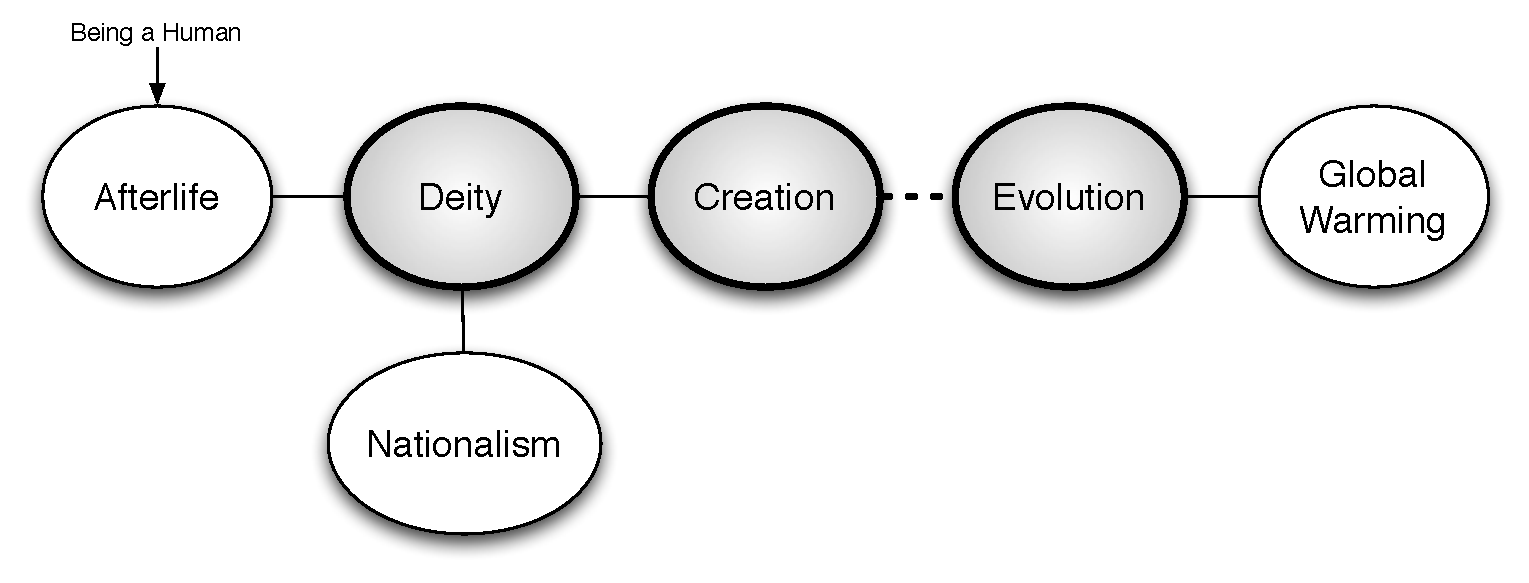
\includegraphics[width=6.5in]{rtmd.pdf}
    \caption{Core RTMD relationships (adapted from \cite{ranney_why_2012}).
        Conceptual reinforcement (operationalized as positive correlation) is
        represented by a solid line, and conceptual incompatability by a dashed
        line. A coherent cluster representing devotion to “god and country” is
        on the left, and a science-accepting cluster is on the right. The most
        direct conflict is captured by the explanatory competition between
        creation and evolution.}
    \label{fig:rtmd}
\end{figure}

\subsection{Na\"ive survey results}

Most of the climate-related interventions that follow include some measure of
participant attitudes and beliefs prior to the intervention. In this
dissertation, we are primarily seeking insight into different forms of
conceptual \emph{change} (and thus, one hopes, behavioral change). Given this, a
detailed consideration of these na\"ive results is beyond our scope. However,
some of the relationships obtained seem relevant to understanding the mind of
our potential students. I thus note such results below. For a fuller treatment
of survey material, please consult the relevant publications of the Reasoning
group (notably, \cite{cohen_san_2012_f,ranney_changing_2012}).

Most importantly, we were able to observe some important relationships from
Cohen’s (\citeyear{cohen_san_2012_f}) data contrary to the “knowledge deficit”
and polarization arguments referenced in Chapter~\ref{chap:intro}. 
% TODO turn the chapter ref into a section when the intro is sorted out.
First, we observe a robust correlation between mechanistic climate change
knowledge and attitude toward climate change.  This result was maintained even
when taking political party into account.  Specifically, mechanistic knowledge
correlates with acceptance that global warming is occurring ($r=0.22$,
$p=0.0002$) and is anthropogenic ($r=0.17$, $p=0.005$).  Anthropogenic climate
change acceptance also predicted financial “willingness to sacrifice” ($χ^2(4) >
32$, $p<0.001$ for each of four items), and one’s knowledge score predicted two
of these items ($χ^2(1) > 3.8$, $p<0.05$ for both). Further, acceptance of
biological evolution was found to predict beliefs and attitudes toward climate
change (as RTMD hypothesizes, and, e.g., \cite{ranney_why_2012} found). We might
infer, then, that “acceptance of controversial science” is a problem above and
beyond political ideology. These findings suggest that the effects of
well-chosen aspects of education are both significant and somewhat independent
of political affiliation. Indeed, evolution acceptance was a significant
predictor of climate change acceptance even in a model including the two major
political parties ($\chi^2(4)=12.3$, $p<0.02$; N.B., including other parties
dramatically reduces quality of fit for any model, likely due to small bin
sizes). Given these results with a representative sample of the american public,
we considered ourselves justified in focusing primarily on attitude and belief
questions in the interventions that follow.

Below, as appropriate, we will see how such relationships maintain
in our various populations in the context of a number of interventions.

% Include multi-correlation figures here?
% 
% Figure? Evo—GW link
% Knowledge / self-knowledge (this isn’t really part of this section)
% Other stuff? Maybe nationalism GW link? How does this tie generally into our
% theoretical framework? How does it compare and contrast with Ranney’s previous
% work?

\section{Study 1: Classroom interventions at UC and UT}
\label{sec:mech-classroom}

This experiment was a fairly thick, exploratory observation of individuals'
beliefs, attitudes and knowledge. Here, “thick” means that we explored the same
phenomenon via multiple routes---for example, doing keyword searches of textual
responses, and examining coded responses via a number of metrics. We sought to
understand how a relatively brief 400-word mechanistic explanation might affect
these measures, as well as how this might be modulated by prior commitment to
one's own explanations and stated attitudes.  The general flow of the experiment
is given in Figure~\ref{fig:mech-flow}.

\begin{figure}[h]
    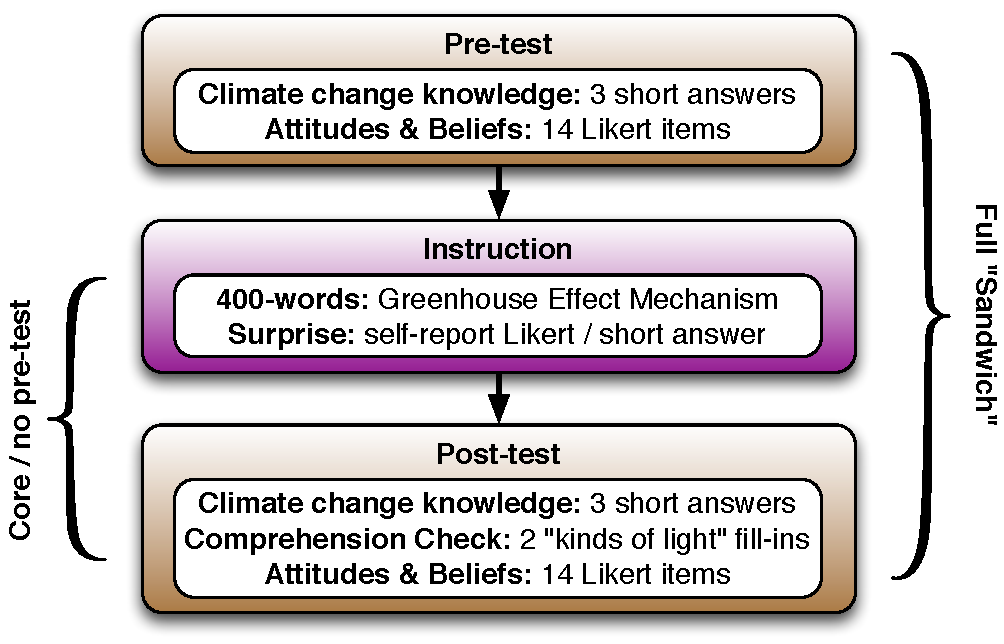
\includegraphics[width=6.5in]{mech-survey-flow1.pdf}
    \caption{An overview of experimental flow for
        Section~\ref{sec:mech-classroom}. Flow for other experiments in
        Chapter~\ref{chap:mechanism} was similar. The analogy to a sandwich
        takes the knowledge and attitutde tests to be slices of bread, and the
        educational intervention itself is the “jam.”}
    \label{fig:mech-flow}
\end{figure}

The primary goal here was a proof of concept. By assessing university
students---some of our nation’s most highly educated citizens---we provide a
strong test of our belief that most Americans are ignorant of the mechanism of
global climate change. An additional concern was that for maximal power, it is
preferable to sample na\"ive beliefs prior to the intervention. In such a
design, we are able to use repeated measures statistics and consequently have
much greater power. On the downside, however, problems can arise from assessment
prior to an intervention. For example, we were concerned that individuals might
exhibit an increase in their stated belief in anthropogenic climate change
merely by dint of experimental demand. This is evaluated via comparison between
our sandwich and no-pretest groups.

As described in Section~\ref{sec:survey}, pre-test responses can be used to
asses na\"ive knowledge and attitudes in the general public. 

% Ryan thinks this is unconvincing, game-show like. Could make a parallel with
% Jame's psychophysical experiments, where people could clearly know that an
% apple is red, but they need to be trained to report the basic visual
% properties of what they see preferentially over reporting "basic level"
% phenomena. The "basic pieces" of our mechanism do indeed seem new to most, but
% we have yet to formally test that part.

\subsection{Experimental Methods}

The general form of the intervention is given in Figure~\ref{fig:mech-flow}, and
was collected anonymously.  Participants were split into two groups, receiving
either the “no-pretest” version of the intervention, or the full “sandwich”
(filled with nourishing descriptions of climate change!). The climate change
knowledge portion of the pre- and post-tests consisted of the three questions
described in Section~\ref{sec:materials}. For this experiment, the likert items
(all on a 1-9 scale) consisted only of \textsf{knwgbl} followed by the first 13
items in Table~\ref{table:rtmd-questions}. Both groups read the educational text
regarding the mechanism of greenhouse gasses (reproduced in full in
Appendix~\ref{app:400words}), and indicated any surprise they may have
experienced (again, on a 1-9 scale). The “kinds of light” check consisted of two
fill-in-the-blank questions regarding the kinds of light coming to earth from
the sun and radiating away. Here, “sunlight” or “visible light” were considered
correct for incoming, and “infrared” was considered correct for outgoing.  Some
participants wrote “ultraviolet” for incoming light, which one could charitably
ascribe to a partially correct understanding.

In addition to the intervention proper described above, participants also
completed a demographic survey, detailed in Table~\ref{table:demographics}.
The experiment began with a page of instructions, including the assertion that
no tricks or deceptions were involved in this study. Lastly, given that their
experimental intervention was shorter, individuals in the “no pre-test” group
were asked to provide some feedback on the intervention, and also on Al Gore’s
“An Inconvenient Truth” (if they had seen it). These responses were used to
refine our methods going forward, and \textcite{bem-future} notwithstanding,
should have had no effect on the results.

\subsubsection{Participants}

% For this intervention, we have collected data from 103 Berkeley undergraduates
% in a single class, and 49 from two classes at the University of Texas,
% Brownsville. Ages? Gender?

103 University of California, Berkeley, and 46 University of Texas, Brownsville,
undergraduates were randomly assigned to one of our two groups: “sandwich” or
“no-pretest.” Below, we report data from the 85 Berkeley and 41 Brownsville
students who completed the survey as intended and had been U.S. residents for
ten years or more (because we expressly consider U.S.
exceptionalism/nationalism). Of the Berkeley data, we analyzed 43 no-pretest
surveys and the pretest part of 42 sandwich surveys---but due to
anticipated time constraints, only 30 sandwich post-tests could be
completed/obtained. Of the Brownsville data, we analyzed 22 no-pretest and 19
complete sandwich surveys.

Of the 85 Berkeley students analyzed, 2 did not complete the demographic test.
43 were female and 40 were male. Mean conservatism was 3.69 (9-point scale; 1.65
standard deviation). Of the 41 Brownsville students 21 were female, 20 were
male. Here, mean conservativism was 4.95 (1.77 $sd$). Political
affiliation is reported in Table~\ref{table:study1-affiliation}.

\begin{table}
    \centering
    \caption{Number of students from both sub-populations stating membership in
        a given political party. Note that the demographic survey was given
        after the intervention (and thus may have influence willingness to state
        party).}
    \label{table:study1-affiliation}
    \begin{tabular}{rcc}
        \toprule
        Party & Berkeley & Brownsville \\
        \midrule
          decline to state &   5  & 7 \\
          democrat &  40  & 7 \\
          independent &   4  & 2 \\
          libertarian &   9  & 1 \\
          none &  24   & 16 \\
          other &   1  & 1 \\
          republican &   2  & 3 \\
        \bottomrule
    \end{tabular}
\end{table}

\subsubsection{Procedure}

Participants were run simultaneously for each of the two classes. Instructions
were administered by the course instructor, and students received one of two
packets---placing them into one of the two groups described above. After
completing the consent form on the front of the packet, individuals proceeded to
read and answer questions. The entire experiment required approximately
25 minutes to complete.

\subsubsection{Analysis}

Handwritten responses were coded and placed into a spreadsheet (for details, see
Appendix~\ref{app:coding}. Given the rich nature of these data, many analyses
were employed. As such, please see the results section that follows for details
of the analysis used for each question.

\subsection{Results}

Please note that all statistical tests are reported in full in the tables
associated with this section. In the text, I primarily indicate only a basic
value to give a sense for the strength of the result.

\subsubsection{Learning the Global Warming Mechanism}

Even our rather sophisticated samples initially exhibited incorrect or
non-normative understandings of the greenhouse effect’s mechanism (e.g., on the
roles of ultraviolet light, the ozone layer’s depletion, nongreenhouse-gas
pollution, and the reflection of incoming light). Most notably, not a single
pre-test explanation mentioned different light/radiation types or atmospheric
retention time, despite an explicit prompt to explain any differences between
the energy traveling toward and away from Earth. However, after reading the
400-word description, 61\% of the Berkeley participants across both groups
correctly answered that “infrared” light was emitted from Earth (in its
fill-in-the-blank space), as did 55\% of the Brownsville students who responded.

Beyond the blank-filling items, we statistically analyzed individuals’
qualitative explanations—creating scoring rubrics for three central concepts:
\begin{description}
    \item[Light] Differentiating between the types of light entering and exiting the
atmosphere 
    \item[GHGs] Atmospheric greenhouse gases’ interactions with radiation
    \item[Energy] The increased atmospheric retention time of energy
\end{description}
Inter-rater reliability
was computed using a weighted modification of Cohen's $\kappa$, described in
full in Appendix~\ref{app:kappa}. This reliability was high (weighted $κ = 0.71$
based on about one-third of the Berkeley data; $κ = 0.67$ across the full
Brownsville dataset). Scores were generated based on three separate aspects of
understanding captured in the coded texts: “Light,” “GHGs,” and “Energy.”
Significant improvements ($p < 0.05$ for all 6 improvement possibilities across
the two groups and three conceptual categories). We had no specific hypotheses,
however, regarding specific effects of a given concept. Therefore, the data
reported below and in Figure~\ref{fig:class-scored-knowledge} use combined
knowledge scores (each sub-score contributes 3 of 9 total possible points).

\begin{figure}
    \centering
    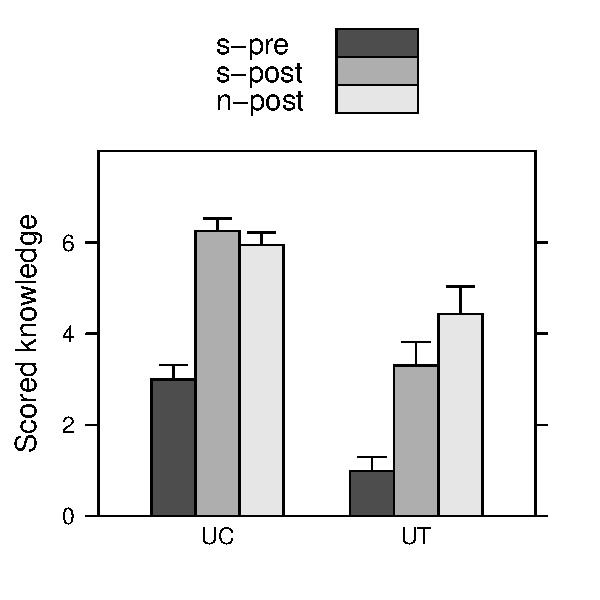
\includegraphics{class-scored-knowledge.pdf}
    \caption{Combined scored knowledge for participants in our classroom
        interventions. All improvements were significant ($p < 0.01$)}
    \label{fig:class-scored-knowledge}
\end{figure}

% TODO: Integrate this into the usage of a figure (get from poster)
% Table 1 shows the per-centages of all possible points: overall, we found
% dramatic knowledge increases (doublings, triplings, or more), which were
% significant for all subscales—both within-subjects for the sandwich condition,
% and between-subjects from the sandwich pretest to the no-pretest condition’s
% posttest, (p < .05 for all six improvement possibilities).  

% TODO: convert this statistic to one using our "good" dataset
Improvements in participant knowledge were readily obtained via different
approaches to analysis. For example, our Berkeley students didn't tend to
mention the mechanism in pre-test (11/42), but they did on the post-test (26/30
for the sandwich group, 39/43 for the no-pretest group).

Participants from both schools experienced significant gains in their self-rated
knowledge after the intervention as well ($p < 0.01$). However, for our
brownsville students in the no-pretest group, they reported a post-test
self-rated knowledge rating almost numerically identical to pre-test ratings in
the sandwich group. And while Berkeley students in the no-pretest group
increased significantly ($p < 0.05$), that increase was numerically smaller than the
sandwich group. These ratings are reported in
Figure~\ref{fig:class-self-rated}.

\begin{figure}
    \centering
    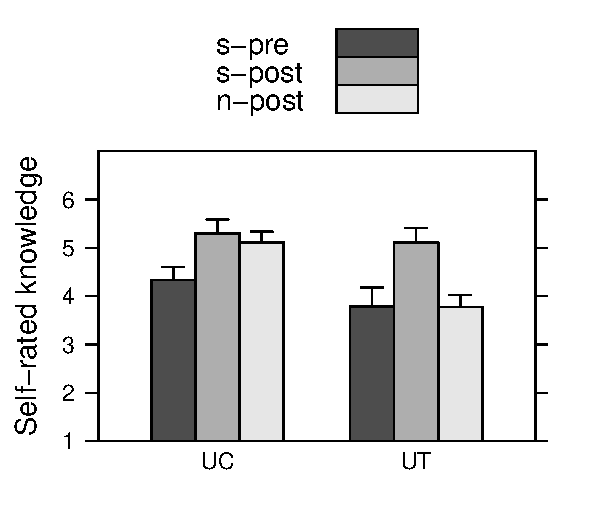
\includegraphics{class-self-rated.pdf}
    \caption{Self-rated knowledge scores for participants in our classroom
        interventions. Improvements in our sandwich groups were significant ($p
        < 0.01$), while improvements for our no-pretest groups were non-existent
        in the Brownsville group, and smaller (but still significant, $p < 0.05$
        in the Berkeley group.}
    \label{fig:class-self-rated}
\end{figure}

\subsubsection{Global Warming Acceptance Via Mechanistic Learning}

To arrive at an easily comparable measure of global warming acceptance, we
averaged together all of the items starting with “gw” used in this study.
\textsf{lifsty} was omitted due to some concerns regarding multiple
interpretation. This concern was in fact unfounded---this construct shifted
similarly to the others---but we retain this set of items throughout our
statistical testing to maintain consistency and genuine \emph{a priori}
hypothesis testing. 

It may seem quite remarkable, but participants’ global warming acceptance
increased dramatically after our brief intervention, as predicted.
Proportionally, participants shifted on average 14\% closer to ``extreme''
agreement with climate change items. To assess this, we used all of the 73
Berkeley post-test ratings in a paired $t$-test, and used imputation for pretest
scores for the no-pretest group. We found a significant change in global warming
acceptance on the posttests, as compared to pre-test measures ($t(72) = 2.28$,
$p = .01$). This result was replicated with the Brownsville surveys ($t(39) =
4.24$, $p < .0001$). These ratings are given in
Figure~\ref{figure:class-gw-ratings}.

\begin{figure}
    \centering
    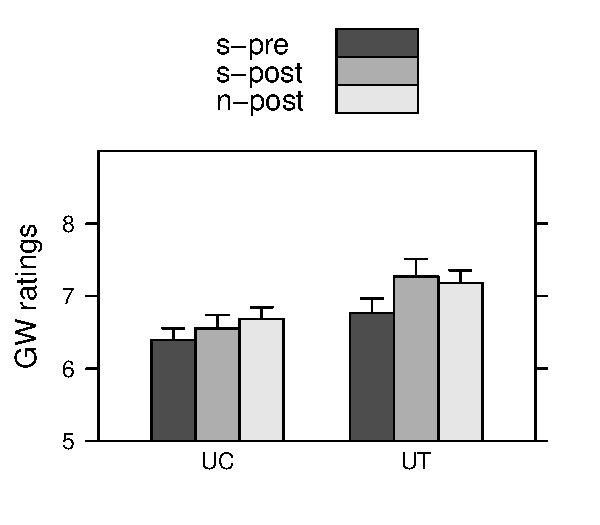
\includegraphics{class-gw-ratings.pdf}
    \caption{Changes in mean of Climate Change related beliefs and attitudes.
        Improvements from pre- to post-test were significant ($p < 0.05$) with
        Berkeley students using a combined $t$-test with imputation.
        Improvements for Brownsville students were also significant using
        imputation ($p < 0.01$), as well as looking only at the sandwich group
        ($p < 0.01$).}
    \label{fig:class-gw-ratings}
\end{figure}

\subsubsection{Predicting Na\"ive GW Beliefs and Attitudes}

% This result is really interesting to me - insert a figure about it!
The relationship between knowledge and attitudes was also reflected in Berkeley
students’ naïve pre-test data, in which participants’ self-perceived ratings of
their own global warming knowledge correlated significantly with their global
warming attitudes ($r = 0.39$, $p = 0.01$). This was not the case with
Brownsville students ($r = 0.15$, $p = 0.55$). This may be reflective of overall
lower self-perceived knowledge by Brownsville students. But consider the
findings above, where we see an even more striking difference in terms of
self-rated knowledge between our Berkeley and Brownsville populations. It seems
that Brownsville students may simply have a much less grounded notion of their
self-knowledge when they are not provided with any context on the matter. The
relationships between self-rated knowledge and GW attitudes are depicted in
Figure~\ref{fig:class-predicting-gw.pdf}.

\begin{figure}
    \centering
    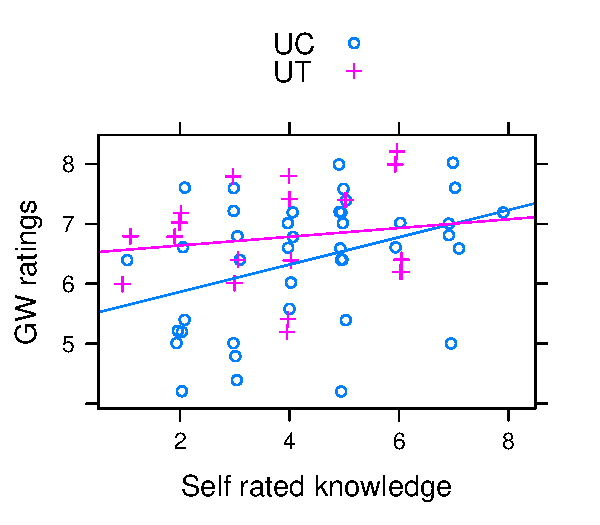
\includegraphics{class-predicting-gw.pdf}
    \caption{Relationship between na\"ive pre-test self-rated knowledge and mean GW
        beliefs and attitudes. This data was only available for participants who
    took the pre-test (i.e., the “sandwich” group). A significant relationship
    obtains for the Berkeley students ($p < 0.01$), while there is very little
    relationship in the Brownsville population.}
    \label{fig:class-predicting-gw}
\end{figure}

\subsubsection{Surprise}

Please recall that we had also predicted a between-conditions difference in
surprise ratings due to reduced hindsight biases among the sandwich
participants. The difference for Berkeley students was at the significance
border-line ($t(42.08) = 1.65$, $p = 0.05$). These surprise ratings increased
from a mean of 2.3 to 3.0 on a 9-point scale. It is a bit of a surprise that
their ratings are so low in general! the surprise ratings only reached “6” in
the no-pretest condition (out of 9, with “5” being “somewhat surprising”), but
were as high as “9” (i.e., “extremely surprising”) in the sandwich condition.
This difference in distribution is depicted in
Figure~\ref{fig:uc-mech-surprise}.  Among Brownsville students, surprise was
uniformly higher, with a numerically similar difference between conditions,
although this result was not significant ($t(38.1) = 0.92$, $p = 0.18$). 

\begin{figure}[h]
    \centering
    \subfloat{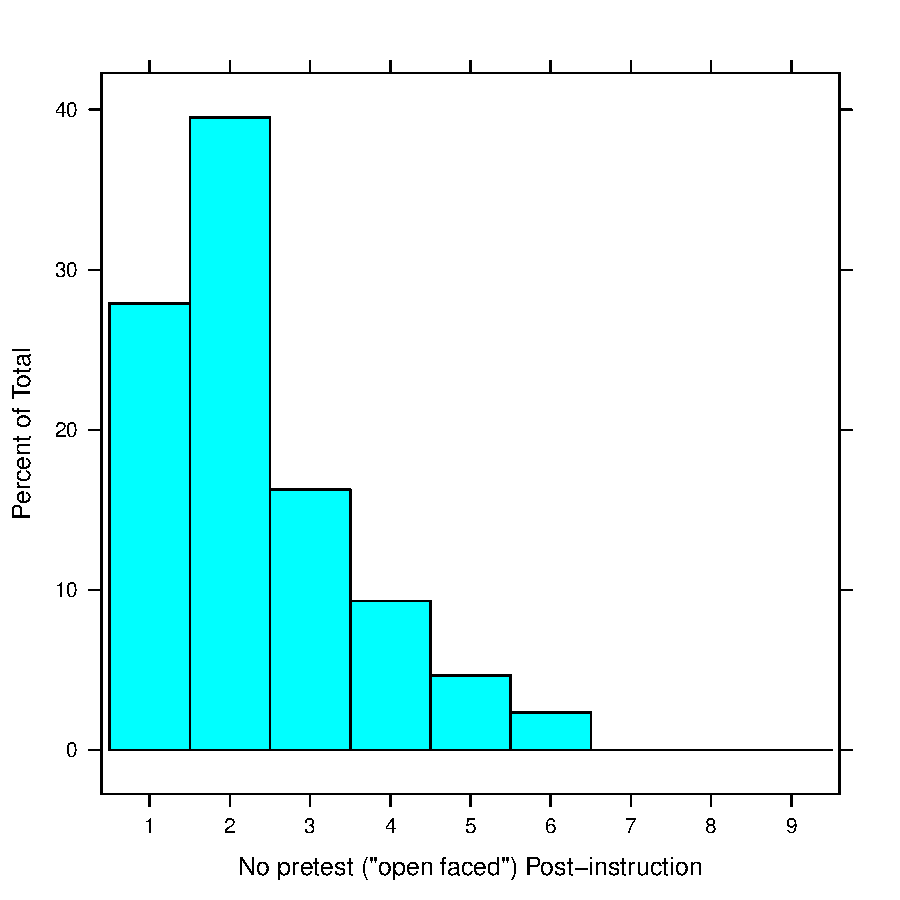
\includegraphics[width=0.5\textwidth]{hypotheses-surprisedistributions1.pdf}}
    \subfloat{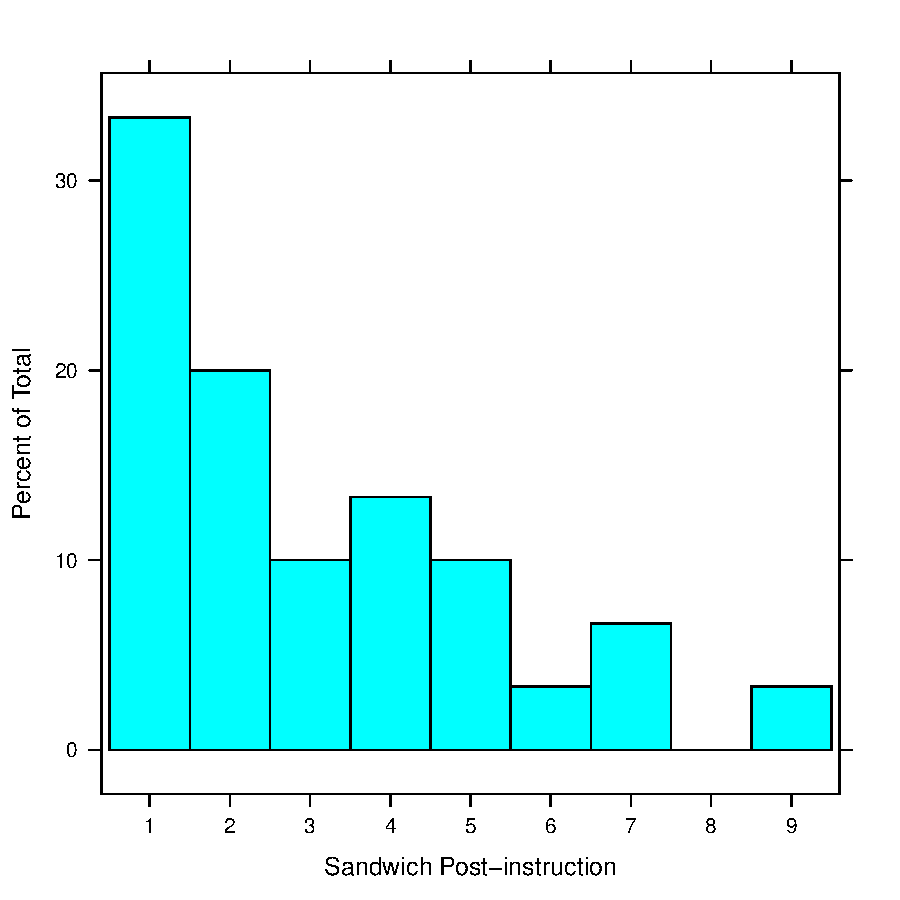
\includegraphics[width=0.5\textwidth]{hypotheses-surprisedistributions2.pdf}}
    \caption{Distributions of surprise ratings for the sandwich and open-faced
        groups, note the slight increase in ``1'' ratings (which may indicate
        resistance to the intervention) co-occurs with an increase (from none)
        in ratings 7-9 in the sandwich group.}
    \label{fig:uc-mech-surprise}
    % For final, re-do these graphs so they have the same y-scales
\end{figure}

Note, I suspect it is unlikely that individuals experienced the same kind of
``visceral'' surprise from the blurb that can be obtained by, for example,
statistics we've used regarding things like abortion and the death penalty. And,
while it may be due to a limitation of imagination, I have even difficulty
imagining an evolution item that would elicit that kind of surprise either.

% In addition, we replicated the relationships predicted by the RTMD theory in
% another population. Confirmatory factor analysis yielded quite similar results
% to simple correlation tables between the means of attitude-relevant items. In
% particular, all proximal relationships held in this population (those
% represented by lines in Figure~\ref{fig:rtmd}) and in each survey, either 12
% or 13 out of 15 total relationships were in the direction predicted by RTMD.
% Less formally, it appears that the correlations between evolution and climate
% change increased after our intervention---perhaps indicating a shift in which
% participants viewed climate change as part of ``real science.'' Similar
% increases in anti-correlation with nationalism were observed. However, we have
% not yet established appropriate statistical machinery to test the significance
% of these effects.
 
% Currently, this is just significant results for the UC CogSci class (2010?)
% from “general improvements”
\extrarowsep 5pt
% copy pasted from mechanism/uc-classroom-summary.csv
% siunitx seems to be doing fine, but you can set it up like this if desired:
% \sisetup{round-precision=2,round-mode=figures,scientific-notation=true}
% I like table-parse-only. This doesn't work somehow: [table-number-alignment = center]
\begin{longtabu}{X[2.5]S[table-parse-only]X[l]}

% Final \\ necessary to compile!
\caption{Summary of “improvement” results for Berkeley classroom interventions.
    All results were \emph{a priori} unless description starts with \emph{“post
        hoc”}.  \label{table:improvements-classroom}}\\ 
\toprule
Result & {$p$-value} & Statistic \\ \midrule
\endfirsthead

% The empty option prevents a TOC entry from being generated
\caption[]{Improvements in Berkeley classroom interventions, continued}\\
\toprule
Result & {$p$-value} & Statistic \\ \midrule
\endhead

\bottomrule
\endfoot

People don't tend to mention the mechanism in pre-test (11/42), but they do in
post-test (S post is 26/30, N is 39/43 -- stat computed for S group pre- vs.
post-, which has a lesser prevalence of mech than N)	&	3.2E-07	&
Fisher's exact "two-sided"	\\
Misconceptions are common in the pretest but not the post test, total 0.38 pre-
to 0.10/0.12 (Sandwich/No-pretest) post-test. Ozone .19 to .03/.02 (S/N),  wrong
GHG  .24 to 0.07/0.09 (S/N). (test on total misconceptions, Sandwich pre- to
group-specific post-test)	&	0.01	&	Fisher's exact "two-sided"	\\
Participants don't mention energy leaving the earth until prompted.
Specifically, of the four codes that deal with this topic, only 6 mention
something about “trapped heat” in the pre-test on the first (i.e., the only
unscaffolded) question.	&	0.0002	&	Fisher's exact "two-sided"	\\
Use of infrared is greater post-test than pre-test. Goes from 0 to 16 / 22 in S
/ N groups.	&	3.5E-08	&	Fisher's exact "two-sided"	\\
Sandwich: GHG Objecive knowledge scores improve after the blurb	&	5.08E-05
&	$t(29) = -4.75$ (paired)	\\
No-pretest: GHG Objecive knowledge scores improve after the blurb	&	2.00E-06
&	$t(78.2) = -5.14$ (Welch)	\\
Sandwich: Light Objecive knowledge scores improve after the blurb	&	3.94E-07
&	$t(29) = -6.51$ (paired)	\\
No-pretest: Light Objecive knowledge scores improve after the blurb	&	1.20E-04
&	$t(79.02) = -4.06$ (Welch)	\\
Sandwich: Energy Objecive knowledge scores improve after the blurb	&	0.04
&	$t(29) = -2.15$ (paired)	\\
No-pretest: Energy Objecive knowledge scores improve after the blurb	&
4.60E-04	&	$t(80.82) = -3.6547$ (Welch)	\\
Differences in GW attitudes are significant	&	0.013	&	$t(72) = -2.28$
(paired / imputed)	\\
Sandwich: pre- to post-test: Increase in self rated knowledge is highly
significant	&	1.40E-05	&	$t(29) = 4.96$ (paired)	\\
No-pretest: post-test (compared to S pre-test) increase in self rated knowledge
is significant	&	0.014	&	$t(78.7) = 2.23$ (Welch)	\\
					
\end{longtabu}


\begin{longtabu}{X[2.5]S[table-parse-only]X[l]}

% Final \\ necessary to compile!
\caption{Summary of individual and group differences for Berkeley classroom
    interventions. All results were \emph{a priori} unless description starts
    with \emph{“post hoc”}.  \label{table:differences-classroom}}\\ 
\toprule
Result & {$p$-value} & Statistic \\ \midrule
\endfirsthead

% The empty option prevents a TOC entry from being generated
\caption[]{Individual and group differences in Berkeley classroom interventions,
    continued}\\
\toprule
Result & {$p$-value} & Statistic \\ \midrule
\endhead

\bottomrule
\endfoot

Surprise is significantly greater in S group than N group	&	0.053	&
$t(42.08)=1.65$ (Welch)	\\
Post-test, slopes (i.e., correlations) between surprise and self-rated knowledge
differ between N group (negative, significant) and S group (which was
numerically positive).	&	0.036	&	$t(69)=2.137$ (interaction term in a
significant linear model)	\\
The no post-test group had a significantly higher word count than the sandwich
group's post-test answers for know1	&	2.5E-4	&	$t(82.91) = -383$
(paired)	\\
No-pretest (post): Females are significantly more accepting of climate change
than males	&	0.048	&	$t(40.19) = -1.71$ (Welch)	\\
There is a significant positive correlation between number of times seeing an
inconvenient truth and warming attitudes	&	0.022	&	$r(41) = 0.309$	\\

\end{longtabu}


\begin{longtabu}{X[2.5]S[table-parse-only]X[l]}

% Final \\ necessary to compile!
\caption{Summary of relationships between variables for Berkeley classroom
    interventions. All results were \emph{a priori} unless description starts
    with \emph{“post hoc”}.  \label{table:relationships-classroom}}\\ 
\toprule
Result & {$p$-value} & Statistic \\ \midrule
\endfirsthead

% The empty option prevents a TOC entry from being generated
\caption[]{Relationships between variables in Berkeley classroom interventions,
    continued}\\
\toprule
Result & {$p$-value} & Statistic \\ \midrule
\endhead

\bottomrule
\endfoot

Surprise is almost significantly positively correlated with change in total
objectively scored knowledge	&	0.047	&	$r(28) = 0.355$	\\
\emph{Post hoc:} There is a significant correlation between self-rated knowledge
and GW attitudes on the pre-test ONLY (differences in self-rated knowledge are
also insigificant). NB: we predicted the opposite result!	&	0.012	&
$r(40) = 0.386$	\\
\emph{Post hoc:} Sandwich: Negative correlation between post-test self-rated
knowledge and CHANGE in objective score	&	0.011	&	$r(28) = -0.458$	\\
\emph{Post hoc:} Sandwich: Interaction term -- reversal in slope for the S group
between scored and self-rated knowledge pre- to post-test	&	0.047	&
$t(68) = -0.324$ (interaction term in a significant linear model)	\\
Carefulness is significantly correlated with posttest GW attitudes.	&	0.035
&	$r(41) = 0.279$	\\
Rereading is significantly correlated with posttest GW attitudes.	&	0.055
&	$r(41) = 0.247$	\\
\emph{Post hoc:} Counter to our initial hypothesis,There is a negative
correlation between re-reading and post-test objective knowledge scores. NB: we
predicted the opposite result!	&	0.019	&	$r(41) = -0.356$	\\

\end{longtabu}


\begin{longtabu}{X[2.5]S[table-parse-only]X[l]}

% Final \\ necessary to compile!
\caption{Summary of “improvement” results for Brownsville classroom
    interventions.  All results were \emph{a priori} unless description starts
    with \emph{“post hoc”}.  \label{table:improvements-classroom}}\\ 
\toprule
Result & {$p$-value} & Statistic \\ \midrule
\endfirsthead

% The empty option prevents a TOC entry from being generated
\caption[]{Improvements in Brownsville classroom interventions, continued}\\
\toprule
Result & {$p$-value} & Statistic \\ \midrule
\endhead

\bottomrule
\endfoot

Differences in GW attitudes are significant	&	1.30E-04	&	$t(38 = -4.02$
(paired / imputed)	\\
Use of infrared is greater post-test than pre-test. Goes from 0 to 7 / 6 in
Sandwich / No-pretest groups respectively (tested only for Sandwich group)	&
8.00E-03	&	Fisher's exact "two-sided"	\\
Sandwich: pre- to post-test: Increase in self rated knowledge is highly
significant	&	0.001	&	$t(18) = 18$ (paired)	\\
Sandwich: GHG Objecive knowledge scores improve after the blurb	&	0.0034	&
$t(18) = 3.38$ (paired)	\\
No-pretest: GHG Objecive knowledge scores improve after the blurb	&
5.8E-4	&	$t(33.2) = 3.81$ (Welch)	\\
Sandwich: Light Objecive knowledge scores improve after the blurb	&	0.0095
&	$t(18) = 2.9$ (paired)	\\
No-pretest: Light Objecive knowledge scores improve after the blurb	&	1.4E-4
&	$t(25.6) = 4.48$ (Welch)	\\
Sandwich: Energy Objecive knowledge scores improve after the blurb	&	0.02
&	$t(18) = 2.5$ (paired)	\\
No-pretest: Energy Objecive knowledge scores improve after the blurb	&
2.9E-4	&	$t(36.8) = 4$ (Welch)	\\

\end{longtabu}

\begin{longtabu}{X[2.5]S[table-parse-only]X[l]}

\caption{Summary of failures to replicate and associated results with Brownsville classroom
    interventions.  All results were \emph{a priori} unless description starts
    with \emph{“post hoc”}.  \label{table:improvements-classroom}}\\ 
\toprule
Result & {$p$-value} & Statistic \\ \midrule
\endfirsthead

% The empty option prevents a TOC entry from being generated
\caption[]{Failures to replicate with Brownsville classroom interventions,
    continued}\\
\toprule
Result & {$p$-value} & Statistic \\ \midrule
\endhead

\bottomrule
\endfoot

No-pretest: post-test increase in self rated knowledge (compared to S pre-) is
not significant	&	0.51	&	$t(31.4) = -0.036$ (Welch)	\\
\emph{Post hoc:} Self-rated knowledge on  post-test is significantly lower for
No-pretest than Sandwich group	&	0.0019	&	$t(36.6) = -3.36$ (Welch)	\\
There is no correlation between self-rated knowledge and GW attitudes on the
pre-test	&	0.55	&	$r(17) = 0.15$	\\
Surprise is not significantly greater in S group than N group	&	0.18	&
$t(38.1) = 0.92$ (Welch)	\\

\end{longtabu}

\subsection{Discussion}

This experiment replicates and extends findings from prior interviews and
Cohen’s (\citeyear{cohen_san_2012}) survey, such that even rather well-educated
people initially held mostly non-normative understandings of global warming’s
mechanism. Only 400 words later, though (roughly the duration of a TV commercial
break), dramatic increases were observed in (1) mechanistic knowledge and (2)
global warming acceptance. Further, the increases were found in divergent U.S.
states and colleges. Certainly, this suggests that this educational
intervention is a reasonable object of study! Differences in surprise ratings
between the sandwich and no-pretest (“open-faced”) groups further support the
notion that eliciting an explanation or theory prior to offering information
increases surprise and reduces post-hoc rationalization and hindsight bias. (On
surprise, see Chapter~\ref{chap:two}; Munnich, Ranney, \& Song, 2007.) A
graphical depiction of the probabilistic relationships we've established so far
are in Figure~\ref{causal-mechanism}.

\begin{figure}
    \begin{center}
        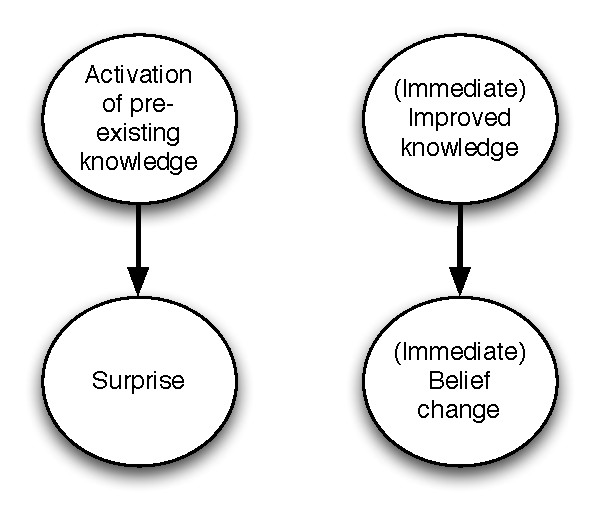
\includegraphics{causal2.pdf}
    \end{center}
    \caption{A graphical model representing the relationship between forms of
        psychological processing of factual information observed in
        chapter~\ref{chap:mechanism}. Here, the relationship between
        pre-existing information and surprise was the result of an experimental
        manipulation and is assumed to be causal. NB: results in the Brownsville
        data were numerically consistent with the significant result found with
        the Berkeley data. Namely, there appears that activating pre-existing
        knowledge boosts surprise.}
    \label{fig:causal-mechanism}
\end{figure}

In addition, we note that there is scant difference between our sandwich and no
pre-test groups in terms of post-test attitudes (with differences going in
opposite directions across our two groups). Thus, it seems unlikely that a
pre-test incurs a greater burden of experimental demand over the core
intervention (400 words followed by a post-test). Moreover, in some populations,
the pre-test may help to anchor self assessment (as with our UT data). And
finally, the sandwich intervention appears to increase reported feelings of
surprise, and likely decreases post-hoc bias. Given these many benefits, in the
work that followed, we standardized on using a sandwich style intervention.

\section{Study 2: A web-based intervention with UC Undergrads}

Given the replicated demonstrations of significant attitude changes described
above, we proceeded to assess whether the mechanism-explanation effects we had
obtained were durable rather than transient. This study extended prior work by
delaying the post-test several days. We also wondered whether an ``experimental
demand'' from the classroom setting might have driven our prior results, so we
provided the intervention on-line; that is, we assessed whether our materials
would elicit significant attitude change even though students participated via
their own computers, without experimenter observation. Thus we concurrently
explored the longevity (via delay) and format (online) aspects of our
phenomenon. We also extended our prompts to incorporate more demographic and
introspection queries.

\subsection{Methods}

The survey and instructional materials were those reported in Ranney et al.
(2012a \& 2012b; the latter includes the full 400-word text of our
intervention). The primary difference was that administration was conducted
entirely online, via the Qualtrics Inc. (Provo, UT) system. Eight items were
added to pre- and post-test attitude surveys to add reliability to the related
RTMD metrics (specifically, national and religious affinities; these metrics
will be reported elsewhere). Five further questions were introduced immediately
following the instructional material to elicit introspection (about
embarrassment, disagreement, etc.).  

Undergraduates (N=80) were recruited via the Research Participation Program
(RPP), administered by the University of California, Berkeley (UCB) psychology
department. Such recruitment allowed us to administer a pre-test to about half
of the students (38) between 8 and 26 days ($\mu=18.5$ days) before any of the
80 participated in the study, which may have allayed test-retest effects
(although Ranney et al., 2012a, found little evidence for them). Thus, as with
Ranney et al. (2012a), some participants received the full survey testing
``sandwich'' while others had no pre-test. A delayed post-test was given to all
participants between 1 and 8 days later ($\mu=4$ days). This range was used to
assess the timecourse of retention in planning subsequent studies, We lack the
power to test forgetting over time here (though numerically, did not observe
any!).

\subsection{Results} 

Note results have changed a bit for Knowledge (both kinds) using
regression and glht. Should also do something more definitive with the GW
attitude data (though this was unchanged for the CogSci paper).

In general and as anticipated, we replicated Ranney et al.’s (2012a) results and
extended them by finding that shifts were retained over the mean (four-day)
delay. 
% Include more verbiage here explaining lme4, Anova and glht
Scored knowledge was comparable to previously tested UC students, rising from
3.8 on pre-test to 6.5 post-test and 6.3 on followup (gains from pre-test were
significant at $p<0.0001$ for both subsequent scores). GW belief ratings (with
higher ratings being more in concert with science’s consensus) increased from a
6.20 pre-test mean to a 6.54 post-test mean ($t(79)=2.5$, $p=0.006$; a healthy
improvement on our 1--9 Likert scales!). Some of this improvement diminished over
the following days, but most was retained: the mean score on the delayed
post-test was 6.44 ($t(79)=1.7$, $p=0.05$). Self-rated knowledge means increased
markedly from pre- to post-test (4.5 to 5.6 on a 9-point scale, $t(79)=8.5$,
$p<0.001$). Retention of this increase, gratifyingly, was also noted on the
delayed post-test (5.2, $t(79)=6.2$, $p<0.001$). (The immediate increase in
self-rated knowledge, in fact, replicates results from the ``sandwich''
interventions in Ranney et al., 2012a, though those results were not reported.)

\subsubsection{Micro-analysis of GW ratings}

Table~\ref{table:uc-online-gw-means} reports the mean rating across participants
for agreement with individual items (For the full text of these items, see
Appendix~\ref{app:survey-items}). The largest gains were found in agreeing with
``Human activities are largely responsible for the climate changes\ldots'' (a
0.25 gain) and certainty that global warming is occurring (a 0.19 gain).  In
general, gains were fairly consistent across all GW measures, ranging only
down to 0.11 at the lowest (the über-greenie “humans are severely abusing the
environment”). Interestingly importance of lifestyle changed the most
(0.27, though this was not included in the tested average gw variable).
Expectation of engagement, dishearteningly, clocks in at a 0.05 \emph{drop}! 
% Enter motivational interventions like Oroeco?

% latex table generated in R 2.15.1 by xtable 1.7-1 package
% Thu May  9 12:43:59 2013
\begin{table}[h]
\caption{Mean GW ratings, online with UC undergrads} 
\label{table:uc-online-gw-means}
\centering
\begin{tabular}{>{\sffamily}rccc}
  \toprule
 & pre-test & post-test & followup \\ 
  \midrule
  gw1\_2 & 6.61 & 6.86 & 6.36 \\ 
  gw2\_1 & 5.19 & 5.31 & 5.25 \\ 
  gw2\_2 & 6.61 & 6.81 & 6.67 \\ 
  gw2\_3 & 5.81 & 5.97 & 5.97 \\ 
  gw2\_4 & 6.78 & 6.86 & 6.67 \\ 
  engage & 5.91 & 5.86 & 6.11 \\ 
  lifesty & 4.83 & 5.11 & 4.94 \\ 
  \bottomrule
\end{tabular}
\end{table}



\subsubsection{Correlations}

Scored knowledge and self-rated knowledge are significantly correlated pre-test,
so participants have decent meta-cognition here.
% TODO: insert statistics from Retention notebook in RPP_Su2012

\subsection{Discussion}

In sum, this study extends the finding that well-considered information, even
received online, increases anthropogenic global warming acceptance and
behaviorally relevant attitudes; the conceptual changes that result from reading
even 400 words have notable longevity. These effects have been replicated with
members of the general public as well (unpublished data). Computer-based
interventions often scale well, enhance reliability, and prove cost-effective;
given our results, we recommend the online distribution of mechanistic
explanations, especially about climate change.  



% New results not in CogSci paper yet

\section{Study 3: A web-based intervention on Amazon Mechanical Turk}

\subsection{Notes to integrate}

A number of additional concerns arise at this point. People may try to take the
survey again, they may lie about their demographics (i.e., claiming they are
U.S. residents so that they may gain the credit), and (bizarrely, as this does
not reduce time required, or increase payment) they may copy and paste from
online sources. Myles (so far) has identified line 14 on his sheet as a problem
in this regard.

\section{Summary and Conclusions}

We've shown across a number of populations that ignorance of the basic
physical/chemical mechanism of the greenhouse effect is nearly universal. In
addition to this research, \textcite{felipe_numerical_2012} describes successes
with a curriculum involving the mechanism with 11th graders (and see
Chapter~\ref{chap:prondi} for more on the numerical estimation aspects of that
study). Across a variety of intervention styles, we have shown that individuals
are able to markedly increase their abilty to describe the greenhouse effect,
and that such an intervention additionally shifts climate-related beliefs and
attitudes.

%TODO - things we can really address with the followup data:

% Look at the relationship between folks saying they learned / were surprised /
% stuff was knew on the basis of their scored knowledge. This is an argument
% against the notion that folks knew things already, but didn’t think to mention
% them given our prompts.

\section{Acknowledgements}

The work reported in this chapter has been previously published, in part, in
\textcite{ranney_improving_2012_f,ranney_changing_2012}, and
\textcite{clark_knowledge_inpress}.  All such material is re-used here with the
permission of my co-authors, the publishers, and the Graduate Division at the
University of California, Berkeley.
